\chapter{Method}

\label{background-information}
Some basic assumptions will apply throughout the modeling of dynamics in thesis. They are as follows:
\begin{enumerate}
\item The vehicle is a fixed mass.
\item Coriolis effects are negligible.
\item Thrust will be assumed to be 0.
\end{enumerate}
Note that a stationary atmosphere is not assumed. The fixed mass assumption is consistent with the electric aircraft used to test the system. At the altitude and speed at which the vehicles will be tested, Coriolis effects can be ignored\cite{klein2006aircraft}. The zero-thrust assumption is in place to minimize drag error. Any error in a measured state will decrease the accuracy of the drag measurement, and the accuracy of the drag measurement can be no better than the worst state measurement error. In-flight thrust is difficult to measure accurately, so a folding propeller will be used, and the motor will be turned off during data acquisition. This will allow the propeller to fold back, eliminating most of the wind-mill drag associated with a stalled propeller. 

\section{Reference Frames}
For this thesis, the reference frames used will follow those described in \cite{klein2006aircraft}, and will be repeated here for clarity.
%todo:make reference frame vector graphics
\subsection*{North-East-Down (NED) Axes ($x_{ned}$, $y_{ned}$, $z_{ned}$)}
The NED axis system defines a local tangent plane on the Earth's surface, with the origin coinciding with the vehicle's center of gravity. The $\hat{i}$ vector points due north, the $\hat{j}$ vector points due east, and the $\hat{k}$ vector points towards the center of the earth, in accordance with the right-hand rule. This coordinate system is vehicle carried, meaning the origin is fixed to the aircraft, but the axis directions are independent of vehicle orientation.

\begin{figure}[h!]
\label{nedAxesFig}
  \centering
    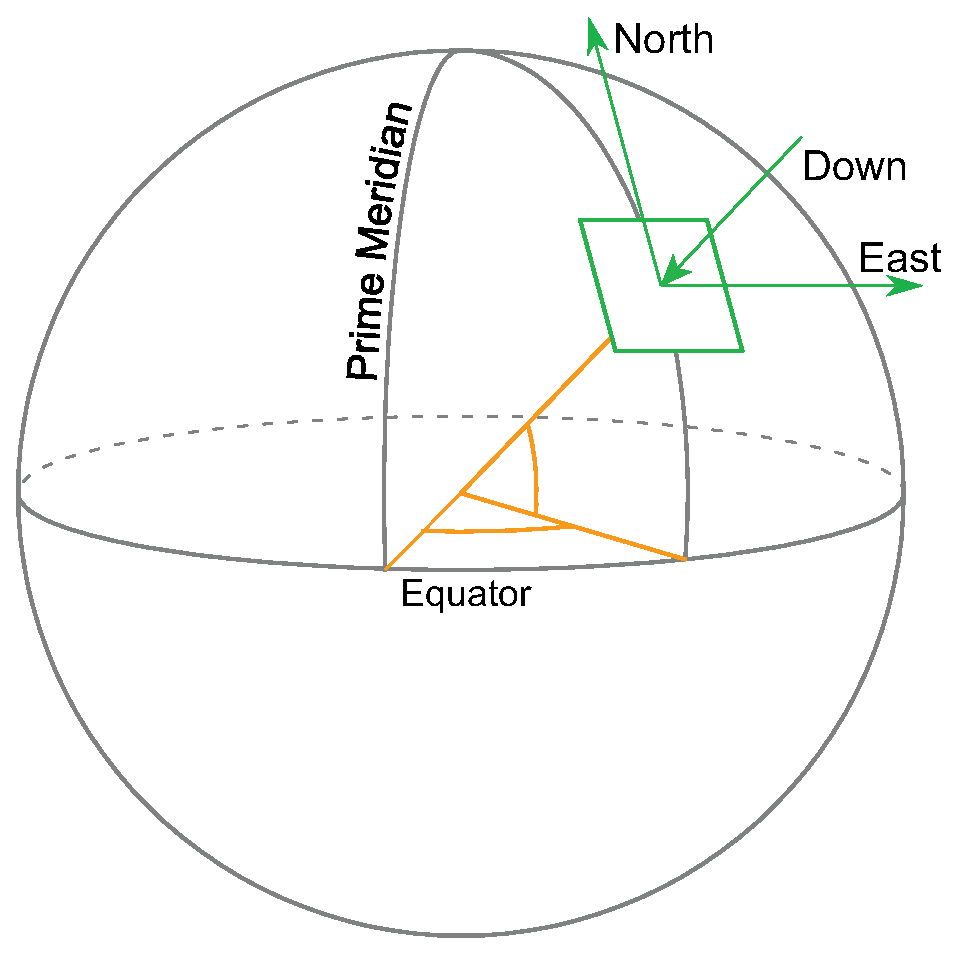
\includegraphics[width=0.4\textwidth]{figures/nedAxes.eps}
      \caption{NED Frame of Reference\cite{nedAxes}} 
\end{figure}

\subsection*{Body Axes ($x_b$, $y_b$, $z_b$)}
The body axis system has its origin at the vehicle's center of gravity, with the $\hat{i}$ direction pointing out the vehicle's nose, the $\hat{j}$ direction pointing out the right wing, and the $\hat{k}$ direction pointing out the belly of the aircraft, in accordance with the right-hand rule. This coordinate frame is fixed to the body, meaning the aircraft's spatial orientation does not change the direction of the axes.
\begin{figure}[H]
  \centering
  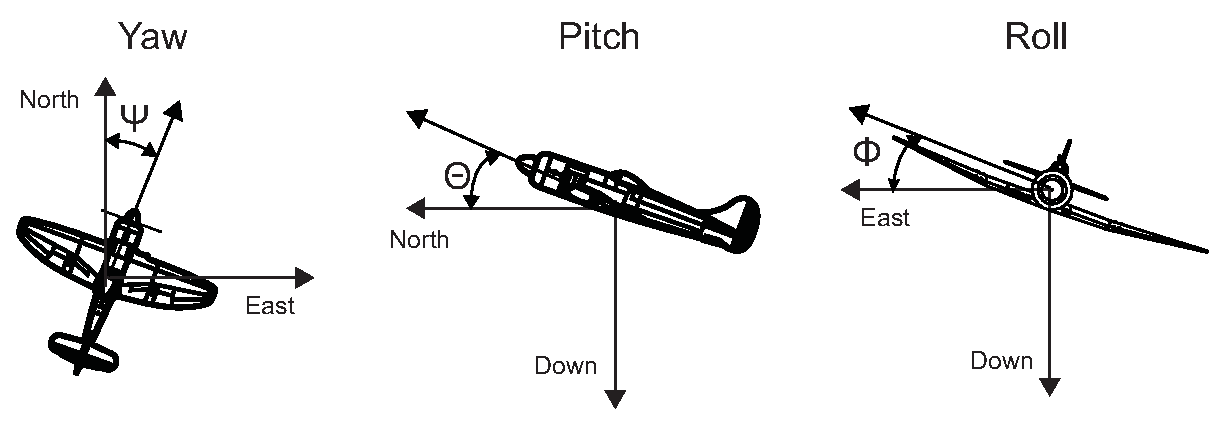
\includegraphics[width=.9\linewidth]{figures/bodyAxes.eps}
  \captionof{figure}{Body Axes Definition\cite{hawkerThreeView}}
  \label{bodyAxesFig}
\end{figure}

\subsection*{Stability Axes ($x_s$, $y_s$, $z_s$)}
The stability axes are defined with its origin coinciding with the center of gravity of the vehicle. This axis system has essentially the same directions as the body axes, except rotated about the body axis $\hat{j}$ through an initial angle-of-attack, $\alpha_{0}$. This inital angle-of-attack is defined at the beginning of a test maneuver and is then set for the remainder of the test, making it a body-fixed coordinate system. This system assumes no initial sideslip angle \cite{roskam2001airplane}. In Figure \ref{stabilityAxesFig}, only the $\vec{i}$ stability vector is shown, for clarity.

\begin{figure}[H]
  \centering
  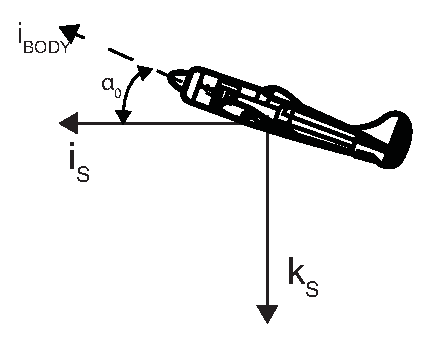
\includegraphics[width=.4\linewidth]{figures/pitchStability.eps}
  \captionof{figure}{Stability Axes Definition}
  \label{stabilityAxesFig}
\end{figure}
\subsection*{Wind Axes ($x_w$, $y_w$, $z_w$)}
The wind axes are, again, a vehicle-carried coordinate system, meaning the origin of the wind axis also coincides with the center of gravity of the vehicle. However, the wind axes are not a body-fixed coordinate frame. The $\hat{i}$ direction points into the oncoming air, as seen from the vehicle. The $\hat{k}$ direction lies in the x-z plane of the body reference frame. The $\hat{j}$ direction is then defined to be out the right side of the vehicle, in order to follow the right hand rule. 

\begin{figure}[H]
  \centering
  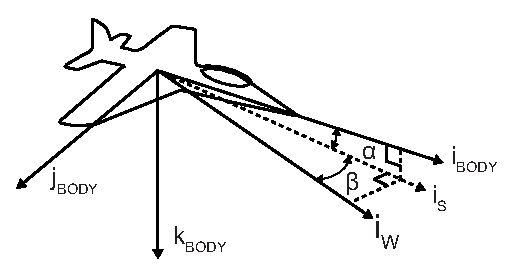
\includegraphics[width=.6\linewidth]{figures/windAxes.eps}
  \captionof{figure}{Wind Axes Definition}
  \label{windAxesFig}
\end{figure}
In Figure \ref{windAxesFig}, only the $\vec{i}$ wind vector is shown, for clarity.

\section{Equations of Motion}
\label{sys-desc}
Newton's 2nd Law of Motion states
\begin{align}
\vec{F} &= \frac{d}{dt}(m\vec{V})
\end{align}
where $\vec{F}$ is the sum of all applied forces, $\vec{m}$ is the mass of the vehicle, and $\vec{V}$ is the vehicle's velocity. Using the fixed mass assumption, this reduces to 
\begin{align}
\vec{F} &= m\frac{d\vec{v}}{dt}\\
&= m\vec{a}
\end{align}

The applied forces on the vehicle are 
\begin{align}
\vec{F} &= \vec{F}_{A}+\vec{F}_{G}+\vec{F}_{T}
\end{align}

where $\vec{F_{A}}$ accounts for all aerodynamic forces acting on the vehicle, $\vec{F_{G}}$ is the force due to gravity, and $\vec{F_{T}}$ accounts for forces from the propulsion system.\\
Aerodynamic forces are described in the stability reference frame. In general, they are defined as

\begin{align}
\vec{F}_{A_S} &= D \hat{i}_s+Y \hat{j}_s+L \hat{k}_s
\end{align}

where $D$ is drag force, $Y$ is side force, and $L$ is lift force.\\
The gravitational force on the vehicle acts in the $+z_{ned}$ direction and is equal in magnitude to the vehicle's weight $W$, leading to
\begin{align}
\vec{F}_{G_{ned}} &= 0\hat{i}_{ned}+0\hat{j}_{ned}+W\hat{k}_{ned}
\end{align}

In general, propulsive forces are modeled as
\begin{align}
\vec{F}_{T_b} &= T_x \hat{i}_b+T_y \hat{j}_b +T_z \hat{k}_b
\end{align}
where $T_x$, $T_y$, and $T_z$ are components of thrust in their respective body axis directions. However, as previously mentioned, propulsive forces are assumed to be $\vec{0}$ for this thesis.\\

The forces are combined and transformed into the body axes reference frame so that they align with the output of body mounted accelerometers. The combined equations of motion are then

\begin{align}
\label{equationsOfMotion}
\vec{F}_{AERO_W} = DCM_{bw}^{-1}(m\vec{a} - DCM_{ib}\vec{F}_{G_{ned}})
\end{align}

The first term in Equation \ref{equationsOfMotion}, $DCM_{bw}$, is a rotation matrix that rotates a vector in body axes into wind axes, through the wind angles $\alpha$ and $\beta$. The vehicle mass and weight are $m$ and $\vec{F}_G$, respectfully. Accelerations are shown by the variable $\vec{a}$. The rotation matrix $DCM_{ib}$ requires the Euler angles between the NED frame and the body frame. These states, when taken together, are the minimum required states for drag polar estimation.

\section{Kalman Filter Usage}
\label{kalman-filter}
This thesis utilizes multiple Kalman filters to estimate both regression coefficients and improved states. As a brief overview, the Kalman filter combines the measured state with a predicted state to give an optimal\cite{kalman60} estimate of the actual system state.

\subsection{Linear Kalman Filter}
A linear Kalman filter can be applied\cite{welch1995introduction} where the system in question can be described in the form 

\begin{align}
x_k &= Ax_{k-1} + Bu_{k-1}+w_{k-1}
\end{align}
where $A$ is the state transition matrix, $x_{k-1}$ is the previous state, $B$ is the input matrix, $u_{k-1}$ is the input vector, and $w_{k-1}$ is random process noise.

The measured state is then 
\begin{align}
z_k &= Hx_k+v_k
\end{align} 

where $H$ is the output matrix and $v_k$ is measurement noise.\\
The Kalman filter operates in a predictor-corrector manner, where the predictor step is often called the \textit{a priori} estimate, and the corrector step is often called the \textit{a posteriori} estimate. The \textit{a priori} state estimate is calculated using prior states and inputs, while assuming no process noise

\begin{align}
\hat{x}^-_k &= A\hat{x}_{k-1}+Bu_{k-1}
\end{align}

The \textit{a priori} estimate of the covariance matrix is projected in a similar manner

\begin{align}
P^-_k &= AP_{k-1}A^T+Q
\end{align}

where Q the process noise covariance matrix.

The Kalman gain is calculated by combining the predicted, \textit{a priori} covariance matrix with the measurement noise covariance matrix $R$

\begin{align}
K_k &=P^-_kH^T(HP^-_kH^T + R)^{-1}
\end{align}

This optimal Kalman gain is then used to estimate the \textit{a posteriori} estimate of the state and covariance matrix

\begin{align}
\label{kalmanStateUpdate}
\hat{x}_k &=\hat{x}^-_k+K_k(z_k-y_k)
\end{align}

\begin{align}
P_k &= (I-K_kH)P^-_k
\end{align}

where $y_k$ is the predicted value of $z_k$ found using the output matrix $H$ and the \textit{a priori} state estimate
\begin{align}
y_k &= H\hat{x}^-_k
\end{align}
Note that Equation \ref{kalmanStateUpdate} is essentially a weighted average of a measured state and an expected state. The weighting is the Kalman gain, which is related to the ratio of confidence in the measured state and the expected state. For a 1-D case with equal confidence between the measured state and the expected state, the Kalman gain $K_k = 0.5$, and the Kalman Filter becomes a simple and straight-forward average.


\subsection{Extended Kalman Filter}
\label{EKFTheory}
The Extended Kalman filter is used for a non-linear system and is essentially a linearization of a nonlinear plant. A non-linear system can be described as \cite{welch1995introduction}

\begin{align}
x_k &= f(x_{k-1},u_{k-1},w_{k-1})\\
z_k &= h(x_k,v_k)
\end{align}

The process noise $w_{k-1}$ and measurement noise $v_k$ are not known (or the Kalman filter would not be necessary), so the states are approximated assuming both noise sources are 0

\begin{align}
\tilde{x}_k &= f(\hat{x}_{k-1},u_{k-1},0)\\
\tilde{z}_k &= h(\tilde{x}_k,0)
\end{align}

The actual states are related to the approximate states by

\begin{align}
x_k &\approx\tilde{x}_k+A(x_k-\hat{x}_{k-1})+Ww_{k-1}\\
z_k &\approx\tilde{z}_k+H(x_k-\tilde{x}_{k-1})+Vv_k
\end{align}

where  the matrices $A$, $W$, $H$, and $V$ represent the different Jacobians matrices:
\begin{align}
A &= \frac{\partial f_i}{\partial x_j}(\hat{x}_{k-1},u_{k-1},0)\\
W &= \frac{\partial f_i}{\partial w_j}(\hat{x}_{k-1},u_{k-1},0)\\
H &= \frac{\partial h_i}{\partial x_j}(\hat{x}_{k},0)\\
V &= \frac{\partial h_i}{\partial v_j}(\hat{x}_{k},0)
\end{align}

The Extended Kalman filter uses these linearized equations to perform the same process as the linear Kalman filter. Again, the first step is to calculate the \textit{a priori} estimate of the state and the covariance matrix
\begin{align}
\hat{x}^-_k &=f(\hat{x}_{k-1},u_{k-1},0)\\
P^-_k  &= A_kP_{k-1}A^T_{k-1}+W_kQ_{k-1}W^T_k
\end{align}

Next, the Kalman gain is calculated
\begin{align}
K_k &=P^-_kH^T_k(H_kP^-_kH^T_k+V_kR_kV^T_k)^{-1}
\end{align}

The Kalman gain is then used to calculate the \textit{a posteriori} estimate of the state and covariance matrix

\begin{align}
\hat{x}_k &=\hat{x}^-_{k}+K_k(z_k-y_k)\\
\label{kalmanVariance}
P_k &=(I-K_kH_k)P^-_k
\end{align}

where $y_k$ is, as in the linear case, the predicted value of $z_k$, but calculated using the nonlinear output function and the \textit{a priori} state estimate

\begin{align}
y_k &= h(\hat{x}^-_k,0)
\end{align}

Unlike the linear Kalman filter, the Extended Kalman filter is not proven to be optimal. However, it has been utilized for a wide range of applications with excellent results.
